\documentclass[a4paper, 12pt]{article}

\usepackage[T2A]{fontenc}
\usepackage[utf8]{inputenc}
\usepackage[english,russian]{babel}
\usepackage{listings}
\usepackage{multirow}
\usepackage{pgfplots}
\usepackage{pgfplotstable}
\usepackage[normalem]{ulem}
\usepackage{geometry}
\usepackage{amsmath}
\usepackage{titlesec}

\usepgfplotslibrary{units}
\pgfplotsset{compat=1.14}
\geometry{left=25mm, right=10mm, top=20mm, bottom=20mm}

\renewcommand{\thepart}{\arabic{part}}
\renewcommand{\thesection}{\thepart.\arabic{section}}


\begin{document}
\thispagestyle{empty}

\begin{center}
    Санкт-Петербургский политехнический университет Петра Великого\\
    Институт Компьютерных Наук и Технологий\\
    \bfseries{Высшая школа программной инженерии}
\end{center}

\vspace{20ex}

\begin{center}
    {
    \LARGE \textbf{КУРСОВАЯ РАБОТА} \\[3ex]
    по дисциплине: «Математические модели» \\
    по теме: «Моделирование процесса параметрической идентификации динамического объекта» \\[3ex]
    Вариант №39
    }
\end{center}

\vspace{40ex}

\noindent Выполнил\\
студент гр.23531/21\hfill
\begin{minipage}{0.7\textwidth}
    \hfill \uline{\hspace{3cm}} \hspace{1.1cm} С.А. Фомин
\end{minipage}

\vspace{3ex}

\noindent Руководитель,\\
доцент\hfill
\begin{minipage}{0.7\textwidth}
    \hfill \uline{\hspace{3cm}} \hspace{0.5cm} Т.В. Леонтьева
\end{minipage}

\vspace{3ex}

\hfill \begin{minipage}{0.6\textwidth} \hfill «\uline{\hspace{1cm}}»\uline{\hspace{3cm}} 2017 г.\end{minipage}

\vfill

\begin{center}
    Санкт-Петербург\\
    2017
\end{center}

\newpage
\thispagestyle{empty}
\begin{center}
    ЗАДАНИЕ\\
    НА ВЫПОЛНЕНИЕ КУРСОВОЙ РАБОТЫ \\[1ex]
    студенту группы 23531/21 Фомину С.А.
\end{center}

\vspace{0.5cm}

\begin{enumerate}
    \item
        \textbf{Тема работы:} Моделирование процесса параметрической идентификации динамического объекта, вариант №39
    \item
        \textbf{Срок сдачи студентом законченного проекта (работы):} 30.12.2017
    \item
        \textbf{Исходные данные к проекту (работе):}
            $$W(s) = \frac{k(1-as)}{(1+as)(1+b_1s+b_2s^2)}$$
            $$
                \begin{matrix}
                    \begin{aligned}
                        x(t) = 5 \\
                        k = 4 \\
                        a = 3 \\
                        b_1 = 1 \\
                        b_2 = 2
                    \end{aligned}
                    &
                    \hspace{3cm}
                    \begin{aligned}
                        \text{метод оптимизации}&: \text{Гаусса-Зейделя $(GZ_1)$} \\
                        \text{целевая функция}&: \text{2} \\
                        \text{шум}&: \text{2} \\
                        \text{считать неизвестными}&: \text{$k, b_1$} \\
                    \end{aligned}
                \end{matrix}
            $$
    \item
        \textbf{Содержание пояснительной записки (перечень подлежащих разработке вопросов):} введение, основная часть (раскрывается структура основной части), заключение, список использованных источников, приложения, нахождение $y^T$, создание и проверка ГСЧ с помощью гистограмм, формирование шума и $y^\epsilon$, реализация алгоритма оптимизации и проверка на тостовых функциях, нахождение $m^M$ и целевой функции $(CF)$, её оптимизация. Примерный объем пояснительной записки 28 страниц машинописного текста
    \item
        \textbf{Консультанты:} Леонтьева Т.В.
    \item
        \textbf{Дата получения задания:} 05 сентября 2017 г.
\end{enumerate}

\vfill

\noindent \textbf{Руководитель} \hfill
\hfill \uline{\hspace{3cm}} \hspace{1.1cm} Леонтьева Т.В.

\vspace{1cm}

\noindent \textbf{Задание принял к исполнению} \hfill
\hfill \uline{\hspace{3cm}} \hspace{1.7cm} Фомин С.А.

\newpage

\part{НАХОЖДЕНИЕ $y^T$}
    \section{Составление системы дифференциальных уравнений}
        $$
            W(s) = \frac{k(1-as)}{(1+as)(1+b_1s+b_2s^2)} = \frac{P(s)}{Q(s)}
        $$
        \vspace{1cm}
        $$
            \begin{cases}
                \dfrac{1}{Q(s)} = \dfrac{u(s)}{x(s)}
                \\\\
                P(s) = \dfrac{y(s)}{u(s)}
            \end{cases}
            \Rightarrow
            \begin{cases}
                y(s) = k(1-as) \cdot u(s)
                \\
                x(s) = (1+as)(1+b_1s+b_2s^2) \cdot u(s)
            \end{cases}
        $$
        \vspace{1cm}
        $$
            \begin{aligned}
                y(s)
                &= k(1-as) \cdot u(s) \\
                &= (k-kas) \cdot u(s) \\
                &= ku(s) - kasu(s)
                \\\\
                x(s)
                &= (1+b_1s + b_2s^2 + as + b_1sas + asb_2s^2) \cdot u(s) \\
                &= u(s) + b_1su(s) + b_2s^2u(s) + asu(s) + b_1as^2u(s) + as^3b_2u(s)
            \end{aligned}
        $$
        \vspace{1cm}
        $$
            \begin{matrix}
                \begin{matrix}
                    x(s) \to x(t) \\
                    y(s) \to y(t) \\
                    u(s) \to u(t) \\
                \end{matrix}
                &
                S = \dfrac{d}{dt}
                &
                S^n = \dfrac{d^n}{dt^n}
            \end{matrix}
        $$
        \vspace{1cm}
        $$
            \begin{aligned}
                y(t) &= ku(t) - ka\dot{u}(t)
                \\
                x(t) &= u(t) + b_1\dot{u}(t) + b_2\ddot{u}(t) + a\dot{u}(t) + ab_1\ddot{u}(t) + ab_2\dddot{u}(t)
            \end{aligned}
        $$
        \vspace{1cm}
        $$
            \begin{aligned}
                \dddot{u}(t)
                &= \frac{1}{ab_2} \cdot (x(t) - u(t) - b_1\dot{u}(t) - b_2\ddot{u}(t) - a\dot{u}(t) - ab_1\ddot{u}(t))
                \\
                &= \frac{1}{ab_2} \cdot \underbrace{(x(t) - u(t) - (b_1 + a)\dot{u}(t) - (b_2 + ab_1)\ddot{u}(t))}_{\Omega}
            \end{aligned}
        $$

    \section{Замена переменных в системе дифференциальных уравнений}
        $$
            \begin{matrix}
                \begin{aligned}
                    z_1(t) = &u(t) &
                    \\
                    z_2(t) = &\dot{u}(t) = \dot{z_1}(t) &
                    \\
                    z_3(t) = &\ddot{u}(t) = \dot{z_2}(t) &
                    \\
                    &\dddot{u}(t) = \dot{z_3}(t) = \Omega &
                \end{aligned}
                &
                \Rightarrow
                &
                \begin{aligned}
                    \dot{z_1} &= z_2
                    \\
                    \dot{z_2} &= z_3
                    \\
                    \dot{z_3} &= \dfrac{\Omega}{ab_2}
                \end{aligned}
                &
                \Rightarrow
                &
                y(t) = kz_1 - kaz_2
            \end{matrix}
        $$

    \section{Решение системы методом Эйлера}
        $$
            \begin{cases}
                z_{1,n+1} = z_{1,n} + h \cdot z_{2,n}
                \\
                z_{2,n+1} = z_{2,n} + h \cdot z_{3,n}
                \\
                z_{3,n+1} = z_{3,n} + h \cdot \Omega
            \end{cases}
        $$
        $$
            y(s) = kz_{1,n} - kaz_{2,n} = k(z_{1,n} - az_{2,n})
        $$
    \newpage
    \section{График и таблица значений}
        \begin{center}
            \begin{tikzpicture}
                \begin{axis}[
                    width=16cm,
                    height=10cm,
                    xlabel=t,
                    ylabel=y(t),
                    minor tick num = 1,
                    grid = both
                ]
                    \addplot table [col sep=comma] {dat/theor.csv};
                \end{axis}
            \end{tikzpicture}
            \pgfplotstabletypeset[
                col sep=comma,
                columns/x/.style = {
                    string type,
                    column name = $t$,
                    precision=1,
                    dec sep align
                    },
                columns/y/.style = {
                    column name=$y(t)$,
                    fixed,
                    precision=11,
                    dec sep align
                }
            ]{dat/theor.csv}
        \end{center}

    \section{Проверка}
        При $x(t) = const (C) = 5$ и $k = 4$
        $$
            \lim_{s\to0}CW(s) = C \cdot \lim_{s\to0}\left(\dfrac{k\overbrace{(1-as)}^{\to1}}{\underbrace{(1+as)}_{\to1}\underbrace{(1+b_1s+b_2s^2)}_{\to1}}\right) = C \cdot k = 4 \cdot 5 = 20
        $$

    \section{Выводы первой части}
        Полученная функция сходится к значению того предела, который был вычислен. Был выбран период наблюдения в 25 точек, так как функция сходится и выполаживается быстро и нет смысла увеличивать их количество и/или размер шага.

\part{ОПТИМИЗАЦИЯ}
    Метод Гаусса-Зейделя ($GZ_1$) сводит задачу поиска наименьшего значения функции нескольких переменных к многократному решению одномерных задач оптимизации, по сути - это постепенное, в многократном цикле, сдвигание к результату по координатным ортам.
    \section*{Алгоритм метода оптимизации $GZ_1$}
        \begin{center}
            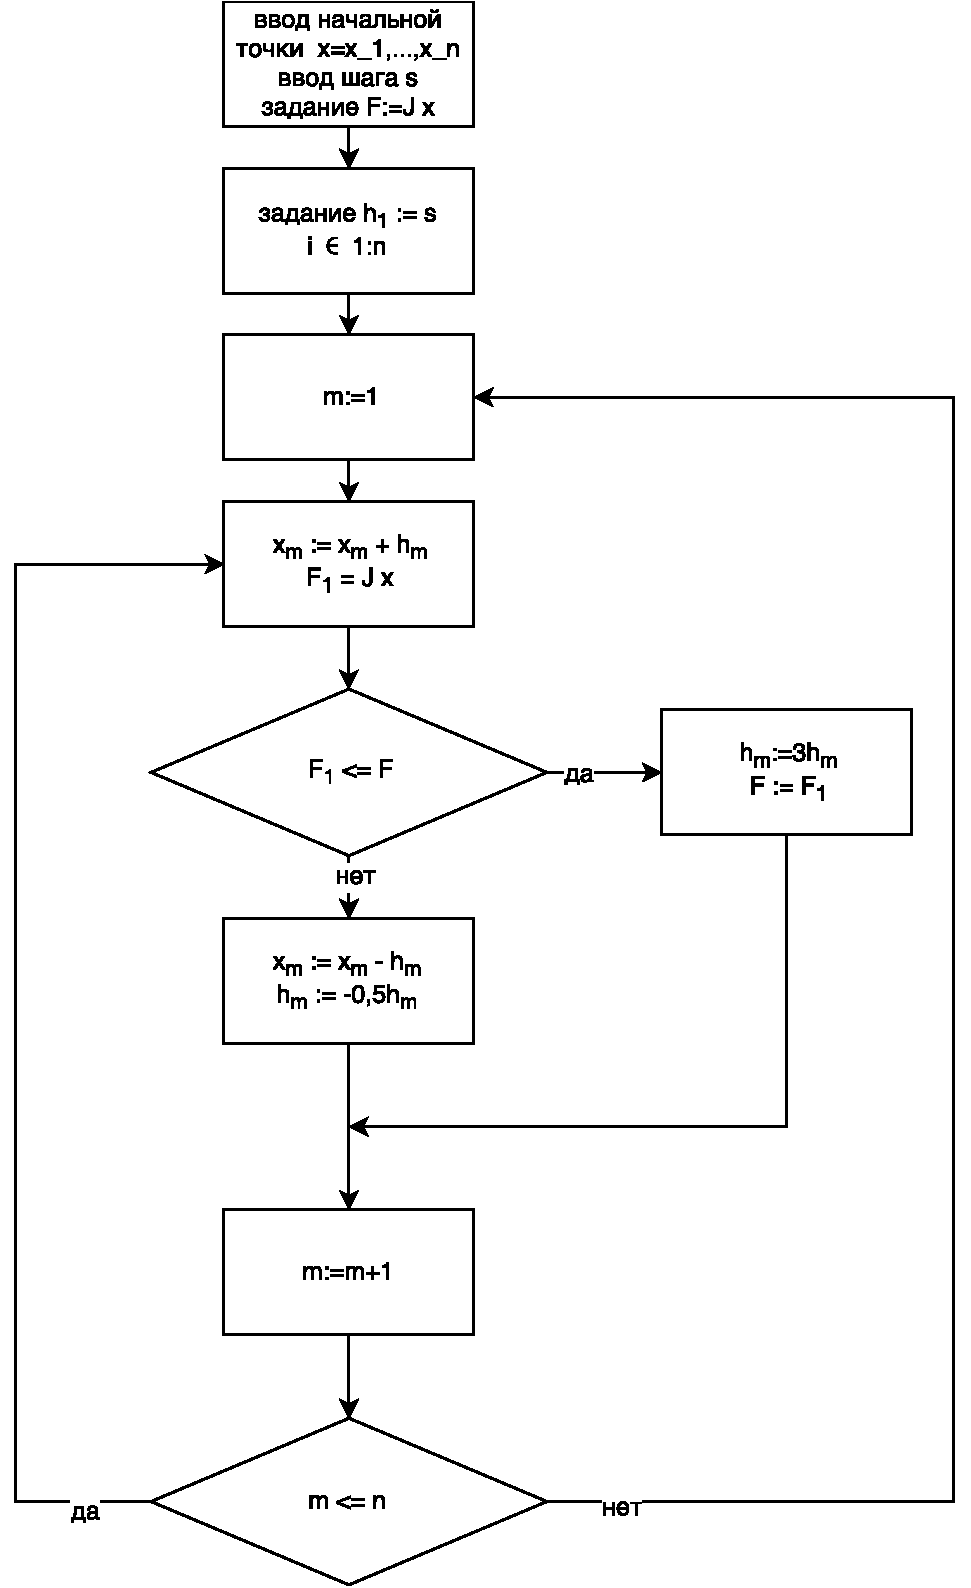
\includegraphics[scale=0.7]{img/gz1-alg}
        \end{center}
        Выход из алгоритма осуществляется по достижении заданного числа вычислений $J$ или при достижении необходимой сходимости.

    \section*{Проверка работоспособности}
        \subsection*{Функция эллипса $r^2 = x^2 + y^2$}
            \begin{tikzpicture}
                \begin{axis}[
                        width=16cm,
                        height=10cm,
                        xlabel=x,
                        ylabel=y,
                        minor tick num = 1,
                        grid = both
                    ]
                    \addplot table [col sep=comma, x index=1, y index=2] {data/ellipse.csv};
                \end{axis}
            \end{tikzpicture}

            Точка минимума $(0;0)$

        \subsection*{Функция Розенброка $z = (1 - x)^2 + 100 \times (y - x^2)^2$}
            \begin{tikzpicture}
                \begin{axis}[
                        width=16cm,
                        height=10cm,
                        xlabel=x,
                        ylabel=y,
                        minor tick num = 1,
                        grid = both
                    ]
                    \addplot table [col sep=comma, x index=1, y index=2] {data/rosenbrock.csv};
                \end{axis}
            \end{tikzpicture}

            Точка минимума $(1;1)$

        Из представленных выше графиков можно сделать вывод о том, что метод оптимизации реализован верно.

\part{ФОРМИРОВАНИЕ ШУМА}
    \section*{Описание процесса формирования шума}
        Интервал распределения шума задан как $ (-\Delta y; \Delta y) $, где коэффициент $\Delta y$ вычисляется по формуле:
        $$
            \Delta y = max(|y^{T}|) \cdot
            \begin{Bmatrix}
                0,05 \\
                0,1 \\
                0,2
            \end{Bmatrix}
            =
            \begin{Bmatrix}
                1.092 \\
                2.184 \\
                4.367
            \end{Bmatrix}
        $$

        После вычисления значений шума, необходимо добавить их к теоретическим значениям в интересующих нас точках для получения экспериментальных значений.

        Можно составить блок-схему процесса генерации экспериментальных значений.

        \begin{center}
            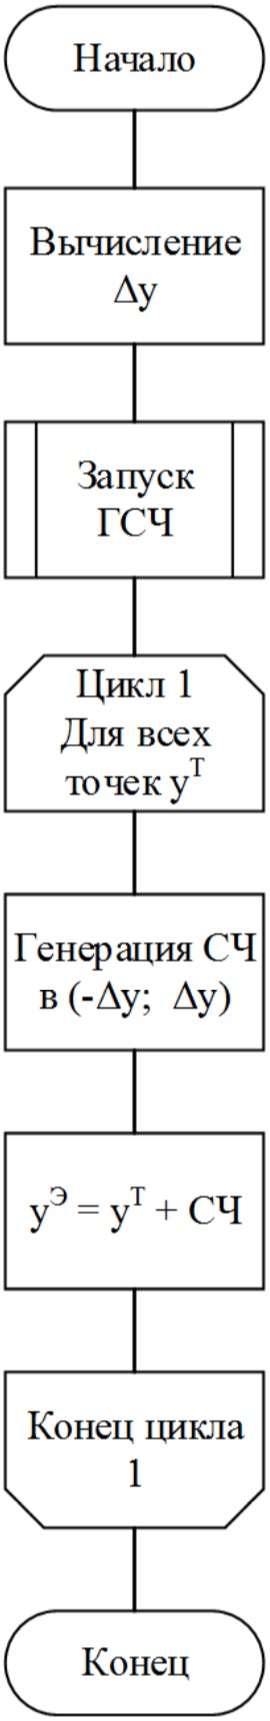
\includegraphics[scale=0.25]{img/block}
        \end{center}

    \section*{Проверка ГСЧ}
        \begin{center}
            \begin{tikzpicture}
                \begin{axis}[ybar, ymin=0, ymax=1200]
                    \addplot [fill, color=blue] table [col sep=comma] {data/rnd.csv};
                    Гистограммы отражают исправную работу ГСЧ.
                \end{axis}
            \end{tikzpicture}
        \end{center}
        Гистограмма выше отражает факт равномерного распределения случайных чисел ГСЧ. Выбран интервал от $0$ до $1$, каждый столбец гистограмы -- интервал, равный $\dfrac{1}{10}$.

    \section*{Построим графики экспериментальных функций}
        \begin{center}
            \begin{tikzpicture}
                \begin{axis}[
                        width=17cm,
                        height=12cm,
                        xlabel=x,
                        ylabel=y,
                        minor tick num = 1,
                        grid = both,
                        legend style={at={(0.5,-0.1)},anchor=north}
                    ]
                    \addplot table [col sep=comma] {dat/theor.csv};
                    \addlegendentry{$Y_{\text{теор.}}$}

                    \addplot table [col sep=comma] {dat/exp1.csv};
                    \addlegendentry{$Y_{\text{Э}}(0.05)$}

                    \addplot table [col sep=comma] {dat/exp2.csv};
                    \addlegendentry{$Y_{\text{Э}}(0.1)$}

                    \addplot table [col sep=comma] {dat/exp3.csv};
                    \addlegendentry{$Y_{\text{Э}}(0.2)$}
                \end{axis}
            \end{tikzpicture}
        \end{center}

\part{ФОРМИРОВАНИЕ ЦЕЛЕВОЙ ФУНКЦИИ}
    \begin{center}
        Целевая функция: $CF=\sum(Y_{\text{э}} - Y_{\text{м}})^2$
    \end{center}

    Неизвестными являются параметры $k$, $b_1$, для оптимизации целевой функции к ней применяется ранее написанный алгоритм. На каждой итерации параметры для расчета нового $y_M$ будут изменяться. Значения остальных переменных остаются такими же, как при вычислении теоретических значений.

    Оптимизация будет выполняться для трех экспериментальных функций $y_{\text{Э1}}, y_{\text{Э2}}, y_{\text{Э3}}$. В результате получаем три пары значений неизвестных параметров.

    \begin{center}
        \begin{tabular}{c|c|c|}
        \cline{2-3}
                                    & k    & $b_1$ \\ \hline
        \multicolumn{1}{|c|}{$CF1$} & 4.16 & 0.938 \\ \hline
        \multicolumn{1}{|c|}{$CF2$} & 4.13 & 0.8   \\ \hline
        \multicolumn{1}{|c|}{$CF3$} & 3.8  & 1.134 \\ \hline
        \multicolumn{1}{|c|}{$y_{\text{сред}}$}   & 4.03  & 0.96   \\ \hline
        \end{tabular}
    \end{center}

    Наложим графики.

    \begin{center}
        \begin{tikzpicture}
            \begin{axis}[
                width=16cm,
                height=10cm,
                samples=1,
                minor tick num = 1,
                grid = both,
                legend style={at={(0.5,-0.1)},anchor=north}
            ]

            \addplot table [col sep=comma] {data/theor.csv};
            \addplot table [col sep=comma] {data/optimized005.csv};

            \end{axis}
        \end{tikzpicture}
    \end{center}

    Так как график, построенный по теоретическим данным практически совпадает с полученным графиком функции с модельными значениями, можно сделать вывод, что оптимизация выполнена верно.


\lstset{
    frame=tb,
    tabsize=4,
    showstringspaces=false,
    numbers=left,
    commentstyle=\color{green},
    keywordstyle=\color{blue},
    stringstyle=\color{red}
}

\newpage
\part*{ПРИЛОЖЕНИЯ}
    \section*{Листинг кода}
        \lstinputlisting{calc.js}

\end{document}
